\section{Regressionsrechnung}
\subsection{Lineare Regression}
\begin{itemize}
	\item Statistische Methode zum Untersuchen und Modellieren der Zusammenhänge zwischen (Mess-)Grössen
	\item $y_i$ ist eine Beobachtung 
	\item $x^{(1)},x^{(2)},\ldots,x^{(m)}$ oder $x_1,x_2,\ldots,x_m$ sind erklärende Variablen 
	\item $y_i$ hängt über eine Funktion $h$ mit den Variablen $x^{(1)},x^{(2)},\ldots,x^{(m)}$ zusammen
	\item Ziel ist des die Funktion $h$ zu finden, sodass diese für jedes $y_i$ gilt
	\begin{itemize}
		\item Eine solche Formel existiert nicht, da es jeweils Abweichungen gibt, also muss sie lauten:
		\item $y_i = h\left(x^{(1)},x^{(2)},\ldots,x^{(m)}\right)+E_i$
	\end{itemize}
	\item $E_i$ ist also der Zufallsfehler (kann von unterschiedlichen Bedingungen, Messungenauigkeiten, etc. abhängige)
	\begin{itemize}
		\item Dieser Fehler muss sich als Wahrscheinlichkeitsverteilung vorgestellt werden
		\item [$\rightarrow$] Normalverteilung mit Erwartungswert 0 und Varianz $\sigma^2 \rightarrow\mathcal{N}(0,\sigma^2)$ 
	\end{itemize}
\end{itemize}
\subsubsection{Transformationen}
\begin{itemize}
	\item Datentransformation kann sinnvoll sein, z.B. Logarithmieren
	\begin{itemize}
		\item So kann $y = C\cdot \frac{x_1}{x_2^2}$ Logarithmiert zu $\log(y) = \log(C)+\log(x_1)-2\cdot\log(x_2)$
	\end{itemize}
\end{itemize}

\subsubsection{Schätzung der Parameter}
\begin{itemize}
	\item Schätzen nach dem Prinzip der kleinsten Quadrate
	\begin{itemize}
		\item Die Summe aller $r_i^2$ soll minimiert werden, siehe Abbildung \ref{fig:reg1}
		\item Die Formel \ref{eq:Reg1} und \ref{eq:Reg2} zeigt die Bestimmung von den Schätzwerten $\hat{\alpha}$ und $\hat{beta}$ 
		\item Dabei ist $\bar{x}$ der Mittelwert aller $x$, dasselbe für $\bar{Y}$
		\item Die Regression berechnet sich aus $n$ Messpunkten
	\end{itemize}
	\item Die geschätzten Parameter $\hat{\alpha}$ und $\hat{\beta}$  treten ebenfalls in der Normalverteilung um ihren Erwartungswert auf
	\begin{itemize}
		\item Somit ist $\hat{\beta}\sim\mathcal{N}\left(\beta,\sigma^{(\beta)2}\right)$ und $\hat{\alpha}\sim\mathcal{N}\left(\alpha,\sigma^{(\alpha)2}\right)$	
	\end{itemize}
\end{itemize}
\begin{figure}[h!]
	\begin{minipage}{0.4\linewidth}
		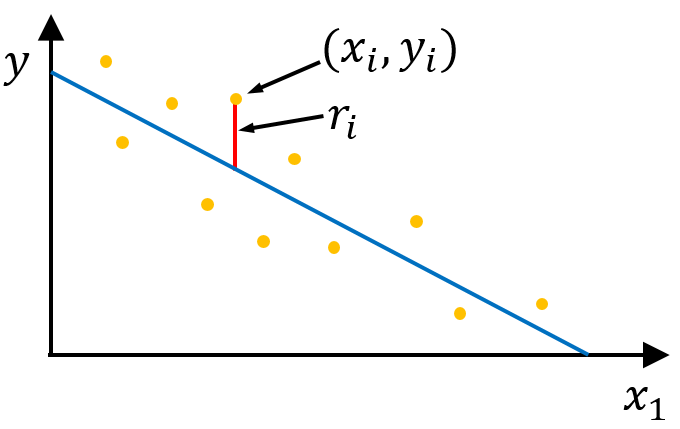
\includegraphics[width=0.8\linewidth]{figures/Reg1}
		\caption{Lineare Regression mit eingezeichnetem Fehler}
		\label{fig:reg1}
	\end{minipage}
	\begin{minipage}{0.7\linewidth}
		\begin{align}
			\label{eq:Reg1}
			\hat{\beta}&=\frac{\sum_{i=1}^{n}\left(\left(Y_i-\bar{Y}\right)\left(x_i-\bar{x}\right)\right)}{\sum_{i=1}^{n}\left(x_i-\bar{x}\right)^2}\\
			\label{eq:Reg2}
			\hat{\alpha}&= \bar{Y}-\hat{\beta}\bar{x}\\
			\label{eq:RegVarianz}
			\hat{\sigma}^2&=\frac{1}{n-2}\sum_{i=1}^{n}R_i^2\\
			\hat{y} &= \hat{\alpha}+\hat{\beta}x
		\end{align}
	\end{minipage}
\end{figure}

\subsubsection{Residuen und Varianzeinschätzung}
\begin{itemize}
	\item Zufällige Fehler $E_i$ können nicht beobachtet werden
	\item Bekannt sind die Näherungswerte für $E_i$ diese heissen \textbf{Residuen}
	\item Fehler Streuen mit Varianz $\text{var}(E_i) = \sigma^2$
	\item Die Schätzung für die Varianz ist in Formel \ref{eq:RegVarianz} gezeigt (neben Abbildung \ref{fig:reg1})
\end{itemize}

\subsubsection{Tests und Vertrauensinterval}
\begin{itemize}
	\item Frage nach möglicher Abweichung zwischen den geschätzten Parametern (z.B. $\hat{\beta}$) und den effektiven Parametern (z.B. $\beta$)
	\item Sind die Daten mit einem Modell  mit (teilweise) vorgegebenen Parametern verträglich?
	\item Definieren einer Nullhypothese, z.B. $H_0: \beta = -2$ wird anschliessend oft mit $\beta^0$ bezeichnet
	\item Gemäss den Formeln \ref{eq:regH0} und \ref{eq:regH01} den T-Wert bestimmen
	\item Diesen Wert T-Wert mit dem T-Wert des festgelegten Niveaus vergleichen (meist 5\%)
	\begin{itemize}
		\item Der Wert des festgelegten Niveau ist in Anh. \ref{Anh:TafelStudentTVerteilung} zu finden
		\item Für 5\%-Niveau die Spalte 0.9750 betrachten!
		\item In Abhängigkeit der Anzahl Datenpunkte
	\end{itemize}
	\item Wenn der berechnete T-Wert kleiner ist als jener der Tabelle: 
	\begin{itemize}
		\item Die Nullhypothese für den gewählten Wert (z.B. $\beta=2$) kann \textbf{nicht} abgelehnt werden
	\end{itemize}
	\item \textbf{Das Vertrauensintervall umfasst alle Punkte deren $H_0$ nicht abgelehnt werden kann}
\end{itemize}
\begin{align}
	\label{eq:regH0}
	T&= \frac{\hat{\beta}-\beta^0}{\text{se}(\hat{\beta})} \qquad \text{mit} \qquad \text{se}(\hat{\beta})=\sqrt{\frac{\sigma^2}{\text{SS}_x}}\\
	\label{eq:regH01}
	\text{SS}_x &= \sum_{i=1}^{n}(x_i-\bar{x})^2
\end{align}

\subsubsection{Vertrauens- und Prognosebereich}
\label{subsubsec:VertrauensUndPrognoseBereich}
\begin{itemize}
	\item Der Vertrauensbereich wird auch als Konfidenzintervall bezeichnet
	\item Oftmals wird hier wieder das 95\%-Vertrauensintervall verwendet 
	\item Die Formeln für die Berechnung des Vertrauensintervall ist \ref{eq:Vertrauensintervall} (für $SS_x$ siehe Formel \ref{eq:regH01}
	\begin{itemize}
		\item der Wert $c_w$ stammt ebenfalls aus Anhang \ref{Anh:TafelStudentTVerteilung}, für 95\% Vertrauensintervall Wert von Spalte 0.975 nehmen, für $n-2$ Freiheitsgrade
		\item Mit dieser Formel erhalten wir die Punkte des Vertrauensintervall oben- und unten an $h(x_0)$ 
		\item Alle plausiblen Werte $\eta$ liegen in diesem Vertrauensbereich und erfüllen somit die Nullhypothese $\eta_0 = \eta_0^o$
	\end{itemize}
	\item Das Vertrauensintervall erklärt nicht in welchem Bereich künftige Beobachtungen zu erwarten sind!
	\item Das Prognoseintervall berücksichtigt zusätzlich noch die Variabilität von $E_i$
	\begin{itemize}
		\item Das Prognoseintervall für die 95\%-Grenze kann gemäss Formel \ref{eq:Prgronoseintervall} berechnet werden
		\item $c_w$ Wert wie zuvor aus Anhang \ref{Anh:TafelStudentTVerteilung}, ebenfalls wieder bei $n-2$ Messungen schauen!
	\end{itemize}
	\item Abbildung \ref{fig:ProgrnoseUndVertrauen} Verdeutlicht das Aussehen dieser zwei Bänder
\end{itemize}
\begin{align}
	\label{eq:Vertrauensintervall}
	\text{Vertrauensintervall} &= \hat{\eta}_\pm c_w \cdot \text{se}\left(\hat{\eta}_0\right) \qquad= \left(\hat{\alpha}+\hat{\beta}x_0\right)\pm c_w \cdot \text{se}\left(\hat{\eta}_0\right) \qquad
	\text{se}\left(\hat{\eta}_0\right) = \hat{\sigma}\sqrt{\frac{1}{n}+\frac{(x_0-\bar{x})^2}{SS_x}}\\
	\label{eq:Prgronoseintervall} 
	\text{Progrnoseintervall} &= \hat{\eta}_0\pm c_w \cdot \sqrt{\hat{\sigma}^2+\left(\text{se}^2\left(\hat{\eta}_0\right)\right)} \qquad= \left(\hat{\alpha}+\hat{\beta}x_0\right)\pm c_w \cdot \sqrt{\hat{\sigma}^2+\left(\text{se}^2\left(\hat{\eta}_0\right)\right)}
\end{align}
\begin{figure}[!h]
	\centering
	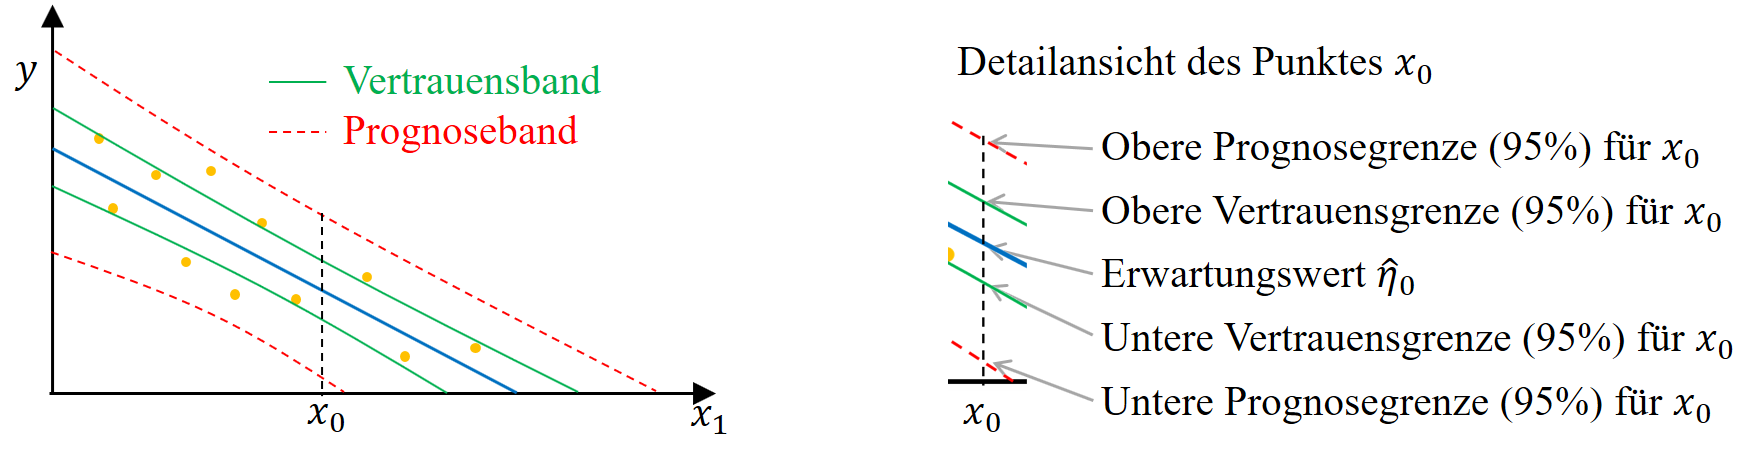
\includegraphics[width=0.7\linewidth]{figures/ProgrnoseUndVertrauensband}
	\caption{Prognose- und Vertrauensband}
	\label{fig:ProgrnoseUndVertrauen}
\end{figure}

\subsection{Prüfen der Modelleignung}
\label{subsec:PruefenModelleignung}
Die Problemstellung ist, dass gewisse Annahmen gemacht werden müssen. Dabei ist die zentrale Annahme, dass die Fehler $E_i$ unabhängig und normalverteilt sind mit konstanter Varianz. $\rightarrow E_i \sim \mathcal{N}\left(0,\sigma^2\right)$  Diese Annahme kann aufgespalten werden in:
\begin{itemize}
	\item Der Erwartungswert $E_i$ ist $E(E_i)=0$
	\begin{itemize}
		\item Punkte Streuen Symmetrisch um lineare Regression
	\end{itemize}
	\item Die $E_i$ haben alle die gleiche Varianz $\text{var}(E_i)=\sigma^2$
	\begin{itemize}
		\item Über die ganze Länge d haben die gemessenen Punkte ($y_i$) in etwa den gleichen Abstand linearen Regressionsgeraden
	\end{itemize}
	\item $E_i$ ist Normalverteilt ($\rightarrow$ Glockenkurve, wenn deren Häufigkeit aufgetragen würde)
	\item $E_i$ sind unabhängig
\end{itemize}

\subsubsection{$R^2$ Bestimmtheitsmass}
\label{subsubsec:R2Bestimmtheitsmass}
Güte der Anpassung der Linearen Regression bestimmen
\begin{itemize}
	\item $R^2\in\left[0,1\right]$ und misst Anteil der durch die Regression erklärte Streung des Y-Wertes 
	\item Quantifiziert den linearen Zusammenhang zwischen den angepassten Werten und den Beobachtungen (quadrierte Korrelation zwischen den Werten)
	\item Je \textbf{grösser} $R^2$ ist, desto \textbf{besser}
	\item Formel \ref{eq:RSquare} Für Berechnung von $R^2$
	\item Quadrat der Summen aller (mit $\alpha$ und $\beta$) geschätzten y-Werte ($\hat{y}$ an den Stellen wo wir ein $y$ haben, dividiert durch das Quadrat der Summe aller gemessenen $y_i$
	\item \textbf{Achtung:} Bestimmtheitsmass gibt keine Auskunft über Eignung des Modells
	\item Das Regressionsmodell erfasst $R^2\cdot 100\%$ der Variabilität in den Zielvariablen
\end{itemize}

\begin{align}
\label{eq:RSquare}
R^2 &= \frac{\sum_{i=1}^{n}\left(\hat{y}_i-\bar{\hat{y}}\right)^2}{\sum_{i=1}^{n}\left(y_i-\bar{y}\right)^2}
\end{align}


\subsubsection{Diagnose Instrumente}
\begin{itemize}
	\item Schwankungen der erwähnte Abweichung (Residuum) zwischen der geschätzten Regressionsgeraden und den gemessenen Punkten  ist von Auge nur schwer zu erkennen
	\item Besser erkennbar wird diese, wenn ein Tukey-Anscombe-Diagramm erstellt wird.
	\item Diese Diagramm trägt die Residuen gegen den Messergebnisse auf.
	\item Eine solches Diagramm ist in Abbildung \ref{fig:residuen} gezeigt.
	\item Von Auge ist die Verletzung der Bedingung \grqq Der Erwartungswert $E_i$ ist $E(E_i)=0$\glqq (siehe \ref{subsec:PruefenModelleignung}) kaum zu erkennen. In diesem Diagramm hingegen ist klar zu sehen, dass die Punkte nicht konstant Symmetrisch um den 0-Wert streuen.
	\item Im Diagramm (Abbildung \ref{fig:residuen}) ist zu erkennen, dass die Residuen nicht immer gleichmässig um 0 Streuen
	\begin{itemize}
		\item Zu beachten ist, dass die Residuen zu den entsprechenden Werte den sie zuvor zugehörten aufgetragen werden (die rote Achse soll dies verdeutlichen).
		\item Hier muss der eingezeichnete gleitende Mittelwert möglichst gleichmässig um die 0-Linie sein (in Diagramm ist zu erkennen, dass dies nicht so ist)
		\item Es liegt also ein Systematischer Fehler vor
	\end{itemize}
	\item Nachfolgend erhalten nur noch die Mittelwerte Beachtung. Wenn immer solche Kurven gezeigt sind, stehen diese für geglättete Mittelwerte
	\item Zur Prüfung ob unsere Residuen sind, erfolgt die Simmulation von 19 Weiteren Messungen. Deren Kurven der gleitenden Mittelwerte der Residuen werden ebenfalls erstellt. 
	\begin{itemize}
		\item Wenn alle diese Kurven  (inkl. der Kurve unserer Linearer Regression) übereinander gelegt werden, muss unsere kurve grossteils im gleichen Bereich verlaufen wie die simulierten Daten. 
		\item Ist dies der Fall: $\Rightarrow$ Die Rote kurve ist typisch
		\item Dieses Vorgehen ist in der Abbildung \ref{subfig:residuen2} gezeigt
	\end{itemize}
	\item Identisch mit diesem Vorgehen kann auch die Eigenschaft $\text{var}(E_i)=\sigma^2=\text{konstant}$ beurteilt werden
	\begin{itemize}
		\item Hier ist wichtig, dass die Kurve möglichst gerade verläuft und nicht zu feste Ausschläge hat
		\item Gezeigt in Abbildung \ref{subfig:residuen3} ist der Verlauf einer Kurve die nicht gut ist. 
	\end{itemize}
	\item Die Voraussetzung das der Fehler normalverteilt ist kann ebenfalls mit einer ähnlichen Methode überprüft werden
	\begin{itemize}
		\item Wird als Normalplot bezeichnet.
		\item Wenn diesr Plot verletzt ist $\Rightarrow$ Normalverteilungsannahme verletzt
		\item Entgegen den zuvor erklärten Methoden werden die simulierten Fehler nicht als Mittelwert aufgetragen, sondern als Messpunkte in den Qunatilen 
		\item Quantile der empirischen Verteilung der Residuen werden mit Quantilen der Normalverteilung verglichen
		\item Punkte streuen um eine Gerade
		\item Im Diagramm werden die Messpunkte der Simulation eingetragen. 
		\item Siehe Abbildung \ref{subfig:residuen4}
		\item Abweichungen dort werden als Langschwänzigkeit oder Kurzschwänzigkeit bezeichnet
		\begin{itemize}
			\item Weglassen des Extremsten Ausreissers kann Abhilfe, schaffen, ist jedoch gefährlich
			\item Robuste Methoden sind in diesem Fall besser als lineare Regression
		\end{itemize}
	\end{itemize}
	\item Sehen diese Diagramme nicht wie gewünscht aus, kann eine Transformation das richten, siehe Kapitel \ref{subsubsec:Transformationen}
	\item Keine \textbf{Evidenz} das Erwartungswert nicht konstant ist $\Rightarrow$ Plot ist gut
\end{itemize}
\begin{figure}[h!]
	\centering
	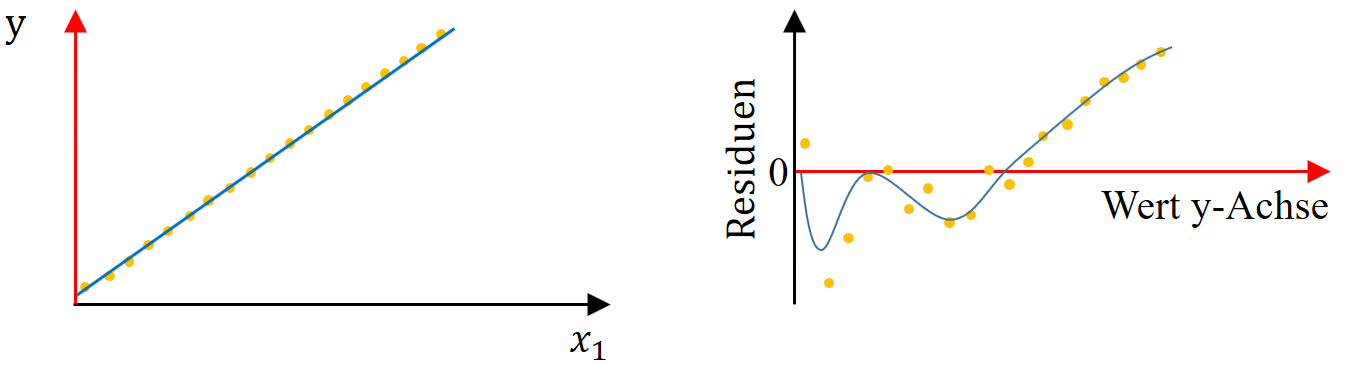
\includegraphics[width=0.6\linewidth]{figures/Residuen}
	\caption{Mit dem Tukey-Anscombe-Diagramm wird die nicht Konstant Verteilung der Residuen ersichtlich. Die gezeichnete Linie wird auch als Glätter bezeichnet}
	\label{fig:residuen}
\end{figure}
\begin{figure}
	\centering
	\subfloat[\label{subfig:residuen2} Tukey-Anscombe-Plot: \textbf{Ist Fehler symmetrisch?}  Resiuduen müssen um 0 sein und innerhalb der grauen beispiel Residuen verlaufen. Kann optimiert werden durch Transformation der erklärenden Variabel]{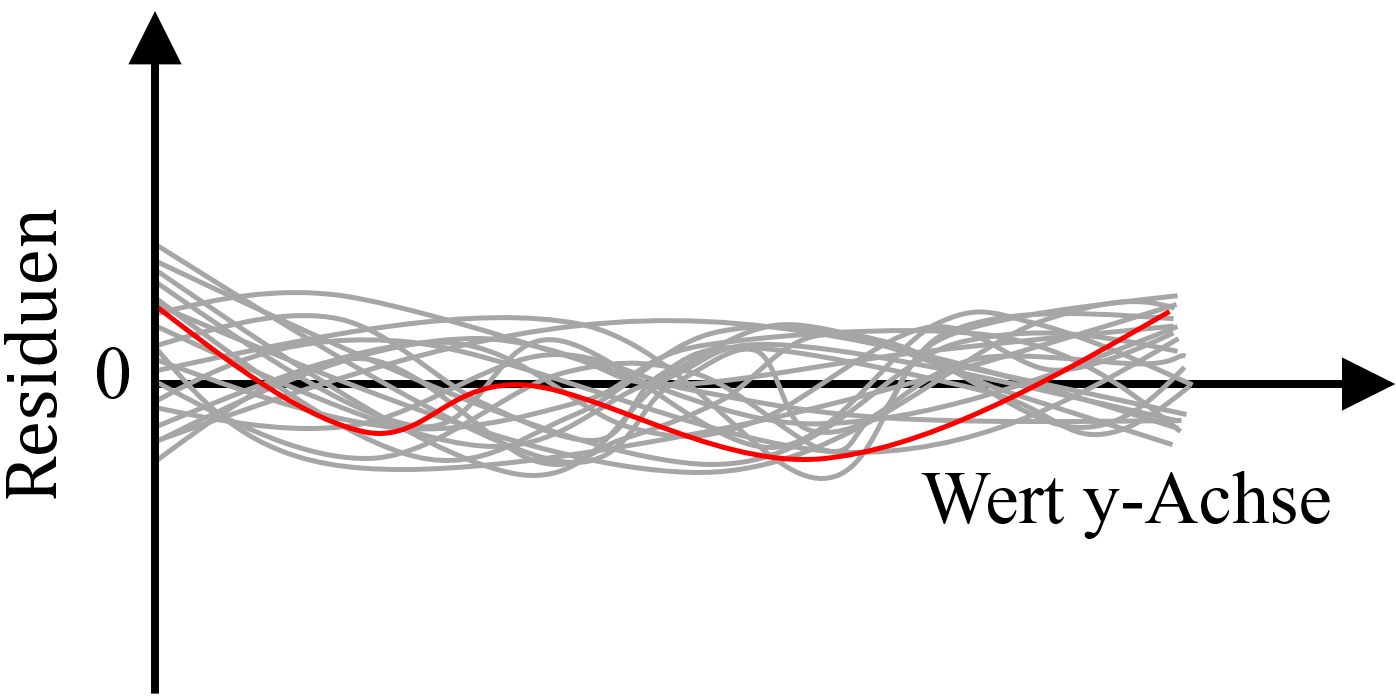
\includegraphics[width=0.25\linewidth]{figures/Residuen2}}
	\hspace{0.1\linewidth}
	\subfloat[\label{subfig:residuen3} Scale-Location-Plot\textbf{Ist Fehler konstant?} Streuung der Residuen muss konstant sein und innerhalb der grauen Beispielstreungen verlaufen, Beispiel zeigt nicht typische Verteilung der Residuen. Kann optimiert werden durch Transformation der Zielvariabel]{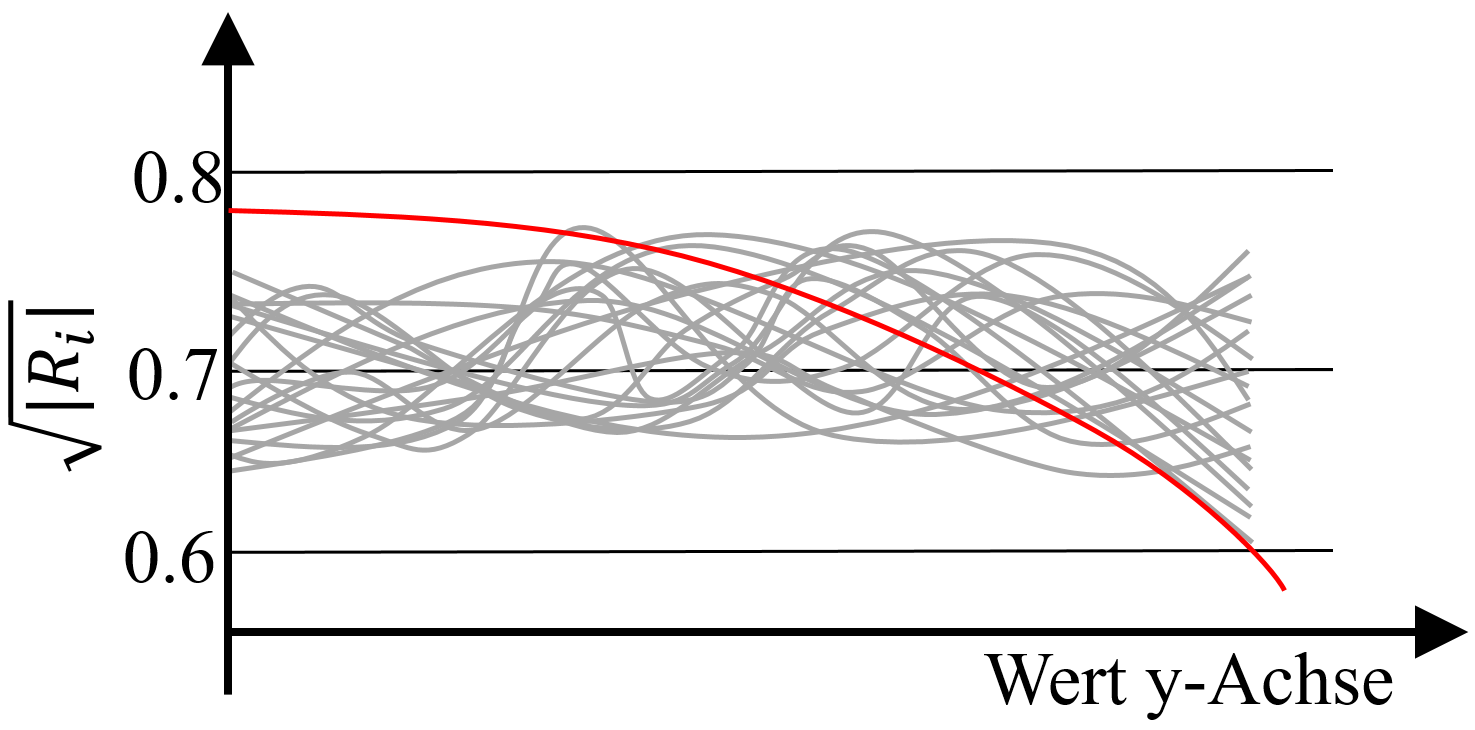
\includegraphics[width=0.25\linewidth]{figures/Residuen3}}\\
	\subfloat[\label{subfig:residuen4} Normal-Plot \textbf{Ist Fehler normalverteilt?} Quantile der empirischen Verteilung der Residuen werden mit Quantilen der Normalverteilung verglichen, \textit{Quelle:}\cite{C:theoQuantilen}]{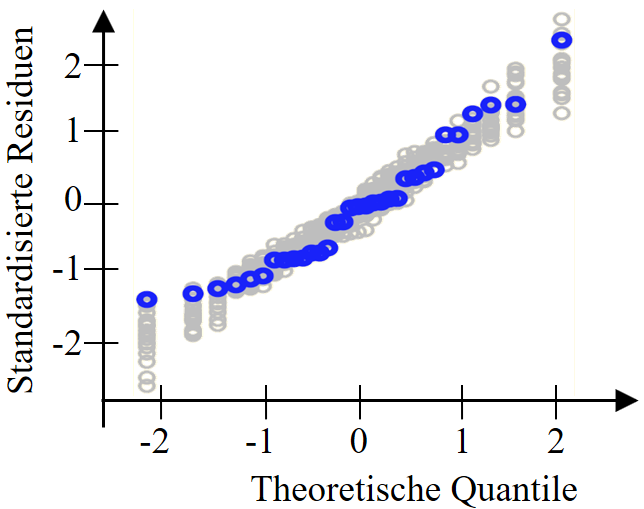
\includegraphics[width=0.2\linewidth]{figures/Residuen4}}
		\hspace{0.1\linewidth}
	\subfloat[\label{subfig:residuen5} Verlauf von langschwänzigen und kurzschäwnzigen Daten]{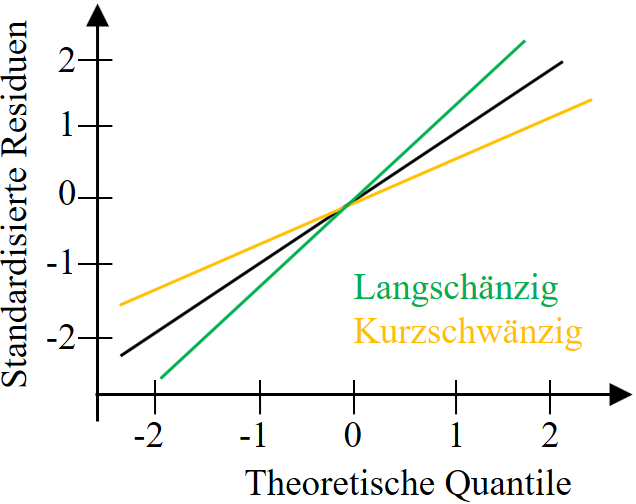
\includegraphics[width=0.2\linewidth]{figures/Residuen5}}
	\caption{Rote Kurven/Punkte müssen innerhalb der grauen Kurven/Punkte verlaufen, dann ist die Form typisch$\rightarrow$ Regression ist gut}
	\label{fig:residuen2}
\end{figure}

\subsubsection{Transofrmationen (Tukey)}
\label{subsubsec:Transformationen}
\begin{itemize}
	\item Diese Empfehlungen beruhen auf Erfahrungen
	\item Die zu verwendende Transformation hängt von dem Typ der Daten ab
	\item Sollen Defizite in der Streuungsannahme beheben
	\item Sowohl auf Ziel variablen, wie auch auf erklärende Variablen Anwenden
	\begin{itemize}
		\item Es können unterschiedliche Transformationen gleichzeitig verwendet werden, wenn z.B. die Erklärende Variabel ein Anteil ist und die Zielvariabel ein Betrag, so kann die Erklärende Variabel mit Arcus-Sinus-Wurzel-Transformation transformiert werden und die Zielvariabel mit der Logarithmus-Transformation.
	\end{itemize}
	\item Die Transformationen
	\begin{itemize}
		\item [1.] Logarithmus-Transformation für \underline{Konzentrationen und Beträge}
		\begin{itemize}
			\item Variablen dürfen kein Zeitlicher Einfluss haben, da diese sonst keine Beträge mehr sind
			\item Beträge: Vorzeichenlose Grössen
			\item Aus $Y_i = \alpha+\beta x_i+E_i$ wird damit $\log_{10}(Y_i) =\alpha+\beta\log_{10}x_i+E_i$
		\end{itemize}
		\item [2.] Die Wurzeltransformation für \underline{Zähldaten} (z.B. Anzahlen) oder wenn etwas mit jeder weiteren Probe abnimmt (z.B. in Folge von Erfahrungsgewinn)
		\item [3.] Arcus-Sinus-Wurzel-Transformation $Y_i = \arcsin(\sqrt{Y_i})$ für \underline{Anteile (Prozentzahlen)} ($\in\left[0,1\right]$)
		\item [4.] Logit-Transformation $y = \log\left(\frac{y+0.005}{1.01-y}\right)$
	\end{itemize}
\end{itemize}

\subsection{Multiple lineare Regression}
\begin{itemize}
	\item Zusammenhang einer Zielgrösse in Abhängigkeit mehrerer Ausgangsgrössen (erklärende Variablen)
	\item $Y_i = \beta_0+\beta_1 x_i^{(1)}+\beta_2 x_i^{(2)}+\ldots+\beta_3 x_m^{(m)}+E_i$
	\item $m =$ Anzahl unterschiedliche erklärende Variablen
	\item $\beta_0 =$ Achsabschnitt, Es gibt nur einen für alle Variablen geltenden Achsabschnitt 
	\item $\beta_m = $ Koeffizient der erklärenden Variabel $x^{(m)}$
	\item $\sigma^2 = $ Varianz der Abweichung $E_i$
	\item Für Beispiels eines R-Outputs siehe \ref{subsubsec:MultipleLineareRegressionR}
	\item Wenn $\text{Pr}(>\vert t \vert)$ kleiner als 0.05 (resp. Vorgegebenem Signifikanzniveau) ist, können wir nicht davon ausgehen, dass das weglassen dieser Variabel keinen Einfluss hat
	\begin{itemize}
		\item Umkehrfolge: Diese Variabel hat einen Effekt auf die Zielgrösse
	\end{itemize}
	\item Es lassen sich keine Schlüsse zum Signifikanzniveau ziehen zwischen einzelnen linearen Regressionen und multiplen linearen Regressionen
	\item Vertrauens, Prognoseintervall und Bestimmtheitsmass genau wie bei einfacher linearer Regression (siehe Gleichung \ref{eq:Vertrauensintervall}, \ref{eq:Prgronoseintervall} und \ref{eq:RSquare})
	\begin{itemize}
		\item $\eta_0 = $ Erwartungswert gemäss Berechnung
		\item $\alpha$ entspricht $\beta_0$, etc.
	\end{itemize}
	\item Polynominale multiple Regression: Wir wählen für $x^{(1)} = x$, für $x^{(2)} = x^2$ etc.  
	\begin{itemize}
		\item Somit können auch Werte von höheren Potenzen mit der normalen linearen Regression angepasst werden 
		\item Formel bleibt somit gleich $Y_i = \beta_0+\beta_1 x_i^{(1)}+\beta_2 x_i^{(2)}+\ldots+\beta_3 x_m^{(m)}+E_i$ 
	\end{itemize} 
\end{itemize}

\subsubsection{Binäre- und Faktorvariablen}
\begin{itemize}
	\item Wie der Name sagt, nimmt entweder Wert 0 oder 1 an
	\item $Y_i =\beta_0+\beta_1x^{(1)}+\ldots+\beta_ix^{(i)}+E_i$
	\begin{itemize}
		\item $x_i$ nimmt für zb. für $i<15$ den Wert 0 an, für Werte $i\geq15$ den Wert 1 an 
	\end{itemize}
	\item Wenn Variabel den Wert 1 annimmt (im Beispiel für $\beta_{15}$ ergibt sich somit: $Y_{15}=\left(\beta_0+\beta_{15}\right)+\beta_1x_{15}^{(1)}$
	\begin{itemize}
		\item Die entspricht also einer Verschiebung des Achsabschnittes um $\beta_{15}$
	\end{itemize}
	\item \textbf{Faktorvariablen} ermöglichen es den Achsabschnitt in Abhängigkeit einer Binären Variabel zu verschieben
	\begin{itemize}
		\item Beispiel: Messungen an verschiedenen Orten des gleichen Ereignisses
		\item Jeder Ort erhält eine Binäre Variabel, die genau dann 1 wird, wenn die Messung von diesem Punkt stammt
		\item Verschiebt den Achsabschnitt genau wie die binäre Variabel 
		\item [$\Rightarrow$] Mit jeder Faktorvariabel geht ein anderer Offset einher
	\end{itemize}
	\item Im Summary-Output entsprechen die $\beta$-Werte der Faktorvariablen gerade der Verschiebung des Achsabschnittes
	\item Faktorvariablen führen zu einem Block von Indikationsvariablen
	\item Siehe für Beispiel Lösung von Übungen Reg3 auf 3b
\end{itemize}

\subsubsection{F-Test (F-Statistik)}
\begin{itemize}
	\item Können alle Variablen zugleich 0 sein?
	\begin{itemize}
		\item Nullhypothese: $H_0: \beta_0 = \beta_1 =\ldots=\beta_m=0$
	\end{itemize}
	\item Wichtig ist, dass der p-Wert der F-Statistik klein ist (<0.05), dann ist 0-Hypothese widerlegt.
	\begin{itemize}
		\item Mindestens einer der Paramter (ohne $\beta_0$ ist ungleich null (und beeinflusst somit die Zielvariabel)
	\end{itemize}
	\begin{itemize}
		\item F-Statistik (...) on x and y DF
		\item x: Anzahl Parameter (ohne $\beta_0$) $\rightarrow$ Anzahl unterschieldiche Steigungen
		\item y: Anzahl Datenpunkte (Anzahl Zeilen der Daten) minus Anzahl der zu bestimmenden Parameter (mit $\beta_0$)
	\end{itemize}
\end{itemize}

\subsubsection{Wechselwirkung}
\begin{itemize}
	\item Wechselwirkung zwischen zwei grössen kann untersucht werden mit:
	\begin{itemize}
		\item \textit{myVar.lm $<-$ lm(A$\sim$X$\ast$Y,data=myDat}
		\item [] \textit{summary(myVar.lm)}
	\end{itemize}
	\item Die Zeile \textit{X:Y (...)} im Output gibt an
	\begin{itemize}
		\item Spalte Estimate: A $\rightarrow$ Steigungsunterschied von X zu Y $\rightarrow$ Wenn $A>0$ hat X eine um A grössere Steigung als Y
		\item Signifikanzlevel: zeigt an bei welchem Signifikanzlevel diese Wechselwirkung signifikant wird
	\end{itemize}
\end{itemize}


\subsection{Sensitivität und Robustheit}

\subsubsection{Senitivität}
\textbf{Cooksdistance}
\begin{itemize}
	\item Wie starkt beeinfflusst eine Beobachtung (insbesondere ein Ausreisser) die Analyse?
	\item Die Distanz von Cook $d_i$ prüft wie fest ein Wert die Schätzung ($\hat{y}_i$) beeinflusst
	\begin{itemize}
		\item Reminder: $\hat{y}_i$ ist der Wert der mit der linearen Regression berechnet wird
		\item Also wird der Einfluss auf die Regressionsgerade (oder Ebene, oder etc.) betrachet
		\item Wert ist normiert mit $p\cdot\hat{\sigma}^2$
	\end{itemize}
	\item Zu einflussreich sind Werte mit einer Cook's Distanz von grösser als 1
\end{itemize}
\textbf{Hebelarm (leverage)}
\begin{itemize}
	\item $h_i$ ist Einfluss der erklärenden Variabel, Wertebereich $0\leq h_i \leq 1$
	\item Die Senitivitätsanalyse mit $h_i$ ist nur bei einzelnen Ausreisser hilfreich, nicht bei Gruppen von Ausreissern
	\item Wenn eine Beobachtung $Y_i$ um $\Delta y_i$ verändert wird, dann ist $h_i\cdot\Delta y_i$ die Veränderung von dem mit der  Regression berechneten Wertes $\hat{y_i}$
	\item Generell gilt, wenn der Hebelarm $h_i<0.2$ ist, ist die Beobachtung unbedenklich
\end{itemize}
\textbf{Punkte identifizieren mit zu grossem Einfluss}
\begin{itemize}
	\item Werden der Hebelarm und die Cooksche-Distanz in einem kombiniert, können damit zu Einflussreiche Punkte identifiziert werden
	\item In Abbildung \ref{fig:sensitivitaet} ist ein solches Diagramm gezeigt, alle standardisierten Fehler $\hat{\sigma_i}$ werden in dieses Eingetragen
	\begin{itemize}
		\item Solange diese Innerhalb der erlaubten Cookschen Distanz (meistens 1) sind ist es kein Problem
		\item Punkte Ausserhalb der Cookschen Distanz haben in y-Richtung einen zu grossen Einfluss
		\item Beobachtungen mit einem Hebel Oberhalb von $h_i>0.2$ haben einen grossen Einfluss auf die Regressionsgerade
		\item Nur Hebelpunkte ($>0.2$) ausserhalb der Cookschen Distanz sind einflussreich
		\begin{itemize}
			\item Solange diese Jedoch innerhlab der Cookschen Distanz liegen sind dies keine Ausreisser und beeinflussen die Regression nicht negativ
		\end{itemize}
	\end{itemize}
\end{itemize}

\begin{figure}[h!]
	\centering
	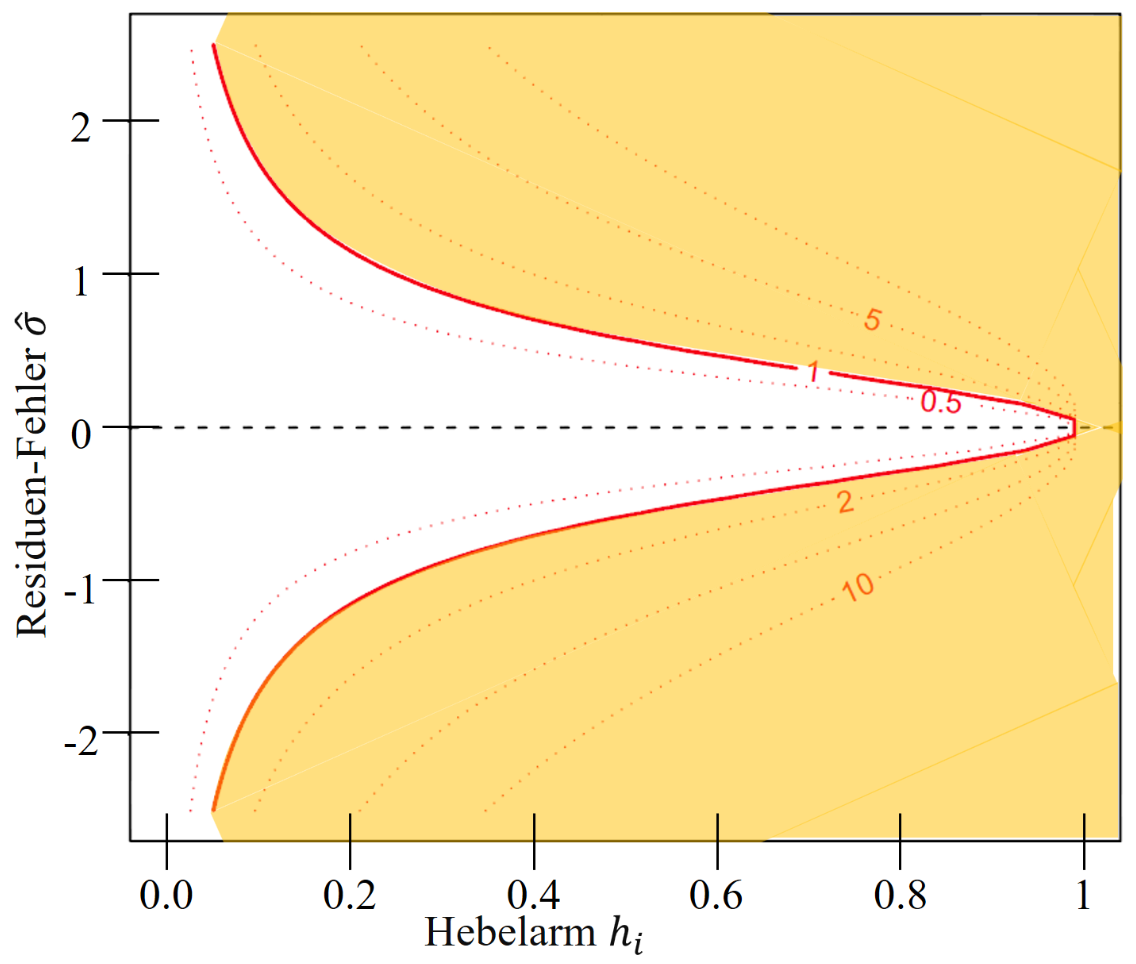
\includegraphics[width=0.3\linewidth]{figures/Sensitivitaet}
	\caption{Sensitivitätsanalyse: Diagramm um Ursache des zu grossen Einflusses zu identifizieren \textit{Quelle: }\cite{C:Cook}}
	\label{fig:sensitivitaet}
\end{figure}

\subsubsection{Gewichtete Lineare Regression}
\begin{itemize}
	\item NoS = Number of Samples
	\item Bei mehreren Beobachtungen denjenigen mit der kleineren Streuung in der Regressionsrechnung das grössere Gewicht geben
	\item \textit{lm(YAches$\sim$XAchse,data = myData, \underline{weights=NoS}}
	\begin{itemize}
		\item Je mehr Samples von einer Probe vorliegen desto grösser wird diese gewichtet
	\end{itemize}
	\item Wenn dies so eingesetzt wird, sollte der zur F-Statistik gehörende p-Wert besser sein, als ohne die Gewichtung.
\end{itemize}

\subsubsection{Robustheit}
\begin{itemize}
	\item Definition von Robustheit
	\begin{itemize}
		\item Ein Ausreisser $P_1$ mit einer kleiner Abweichung von der Normalverteilung hat nur eine kleine Auswirkung auf das Modell
		\item Ein Schätzverfahren, dass die Parameter so schätzt als wäre keine Abweichung vorhanden, wird robust oder resistent genannt
	\end{itemize}
	\item Ein Alter und nicht formeller Ansatz für Robustheit ist:
	\begin{itemize}
		\item Prüfen der Daten auf Ausreisser, diese Ausreisser löschen und Anschliessend modell mit dem verkleinerten Datensatz erstellen
		\item Kein sauberer Ansatz, da es schwer bis unmöglich sein kann Ausreisser als solche von regulären Daten auseinander zu halten. Weiter ist es schwer diesen Prozess zu formalisieren. Weiter Punkte auf Folie 16 von Reg4
	\end{itemize}
\end{itemize}

\subsubsection{Robuste Schätzer (MM-Schätzer)}
\begin{itemize}
	\item Robust Schätzer sollen die Koeffizienten so errechnen, dass Anforderungen an Robustheit und Sensitivität erfüllt werden
	\item \textit{rlm(YAchse$\sim$XAchse, data=myData)} ist ein Robuster Schätzer, aber
	\begin{itemize}
		\item Dieser Berücksichtigt keine Hebelpunkte, sondern korrigiert nur zu grosse Residuen
	\end{itemize}
	\item \textit{lmrob(YAchse$\sim$XAchse, data=myData)} ist ein Robuster Schätzer. 
	\begin{itemize}
		\item Kann sowhol mit grossen Residuen als auch mit Hebelpunkten umgehen
		\item Für Code interpreatation siehe \ref{subsubsec:RobSchaetzer}
	\end{itemize}
	\item Schätzungen mit den kleinsten Quadraten sind ebenfalls ungeeignet, wenn kontaminierte Beobachtungen vorliegen
	\item \textbf{Achtung:} Die Schätzung mit den kleinsten Quadraten kann gut aussehen. Obwohl die Daten ungeeignet sind. In diesem Fall, würde das Auffallen im Robusten Schätzer. Werden die schlechten Daten für die kleinst-Quadrate Methode weggelassen, ergibt diese dann das Gleiche wie der Robuste Schätzer. Andernfalls weisen die Koeffizienten $\beta_m$ massive Abweichungen auf. 
\end{itemize}

\subsection{Variablenselektion}
\begin{itemize}
	\item Nur im Idealfall ist bekannt, das $Y$ von den gegebenen Variablen linear abhängig ist
	\item Im anderen Fall muss der Zusammenhang zwischen $Y$ und den Variablen zuerst hergestellt werden
\end{itemize}

\subsubsection{Adjusted $R^2$, Modellwahlkriterien}
\begin{itemize}
	\item Variabelselektion beruht auf Kriterien, die Güte durch eine statistische Messzahl beschreiben. 
	\begin{itemize}
		\item Diese sollte einerseits Modellgenauigkeit und die Modellkomplexität beschreiben
		\item Komplexität: Wie viele Parameter müssen ermittelt werden
		\item Das sind zwei gegensätzliche Anforderungen
	\end{itemize}
	\item $R^2$ ist eine untaugliche Zahl um als Modellwahlkriterium, da die Modellkomplexität nicht berücksichtigt wird
	\item Das korrigierte Bestimmtheitsmass \textit{Adjusted }$R^2$ trägt dem Rechnung. Berechnet gemäss Formel \ref{eq:AdjR2}
	\begin{itemize}
		\item Dabei ist $n$ die Anzahl der Beobachtungen (Anzahl der Datenpunkte)
		\item und $p$ ist die Anzahl unbekannte Paramter ohne $\sigma$ also Anzahl der $\beta$ (inkl. $\beta_0$)
		\item Achtung: Wenn berechnet werden muss, in Output ist bereits $R^2$ gegeben, nicht mehr quadrieren für Term $1-R^2$
	\end{itemize}
\end{itemize}

\subsubsection{AIC-Kriterium}
\begin{itemize}
	\item bestes verallgemeinertes Kriterium
	\item Formel \ref{eq:AIC} für Berechnung, dabei gilt
	\begin{itemize}
		\item $p^\diamond$  Anzahl geschätzte Parameter (inkl. $\sigma$)
		\item $SS_E$ Summe der quadrierten Residuen
		\item $n$ Anzahl der Beobachtungen
	\end{itemize}
	\item R! versucht wählt jeweils die Option die den AIC-Wert so weit wie möglich ins minus bringt
	\begin{itemize}
		\item Sobald im Output der Wert \glq none \grq den kleinsten Wert hat, wird suche abgebrochen
		\item Beispiel für Schrittweise Selektion in Kapitel \ref{subsubsec:AIC} (Abbildung \ref{fig:aic})
		\item Der default-Wert für die Richtung von step ist \glqq backward \grqq
	\end{itemize}
\end{itemize}
\begin{align}
	\label{eq:AdjR2}
	R_{adj}^2 &=1-\frac{n-1}{n-p}\left(1-R^2\right)\\
	\label{eq:AIC}
	\text{AIC}&= -2\text{(maximierte Log-Wahrscheinlichkeit)} +2\text{Anzahl geschätzte Parameter}
			  &=n \log\left(\frac{1}{n}SS_E\right)+2p^\diamond+Konstante
\end{align}



\subsubsection{Methoden zur Variablenselektion }
\begin{itemize}
	\item Modellwahl: Wahl mit welchen Variablen unser Modell gemacht wird
	\item Achtung: Alle Modellwahlkriterien garantieren nicht das global optimale Modell zu finden
	\begin{itemize}
		\item Der einzige Weg dieses zu finden, ist alle möglichen Kombinationen durchzuprobieren.
		\item All-Subset Selection
		\item Wenn das $m$ (Anzahl der erklärenden Variablen) gross ist, ist Rechenaufwand dafür riesig
	\end{itemize}
	\item Es sollten immer mehrere Modell in Betracht gezogen werden, welche von den Kriterien als gut bewertet sind
	\begin{itemize}
		\item Meist ist das an den Kenngrössen (z.B. $R_{adj}^2$) gemessene, zweitbeste Modell nicht viel schlechter als das\glqq beste \grqq
		\item Es heisst nicht, das das Modell mit dem grössten $R_{adj}^2$ das \glqq wahre \grqq Modell ist.
	\end{itemize}
	\item \textbf{Vorwärtselektion}
	\begin{itemize}
		\item Anfangsschritt: $Y_i=\beta_0+E_i \Leftrightarrow$ \textit{lm(Y$\sim$ 1,...)}
		\item Nehme jeweils diejenige Variabel in das Modell, die zur grössten Verbesserung (Vergrösserung) von $R_{adj}^2$ führt
		\item Stoppregel: Sobald keine Verbesserung mehr erfolgt durch hinzunehmen der nächsten Variabel (alle durchprobieren!)
	\end{itemize}
	\item \textbf{Rückwärtsselektion}
	\begin{itemize}
		\item Beginne mit einer Linearenregression mit allen Variablen \textit{lm(Y$\sim$.,...)}
		\item Lasse jeweils diejenige Variabel vom Modell weg, sodass die zur grösste Verbesserung (Vergrösserung) von $R_{adj}^2$ erreicht wird
		\item Stoppregel: Sobald keine Verbesserung mehr erfolgt durch weglassen der nächsten Variabel (alle durchprobieren!)
	\end{itemize}
	\item \textbf{Schrittweise Selektion}
	\begin{itemize}
		\item Kombination aus Vorwärtsselektion und Rückwärtsselektion.
		\item Bei jedem Schritt probieren, ob das Hinzunehmen oder das Weglassen einer Variablen zum bessern Ergebnis führt
		\item Immer das mit dem besten Ergebnis umsetzen
		\item Stoppregel: Keine Verbesserung mehr möglich
	\end{itemize}
\end{itemize}

\subsubsection{Kollinearität}
\begin{itemize}
	\item Definition: Eine Erklärendevariabel lässt sich als Summe anderer erklärender Variablen darstellen
	\item Hohe Kollinearität zwischen erklärenden Variablen sind von der Theorie her zugelassen, geben jedoch beim Interpretieren und statistischen Modellieren des Modells Probleme
	\begin{itemize}
		\item Bei obigen Verfahren (Vorwärtsselektion, etc.) kann es vom Zufall abhängen, welche Variabel als erstes gewählt wird
	\end{itemize}
	\item \textbf{Variance inflation factor (VIF)} ist das Mass das Aussagen über die Kollinearität zu den anderen Variablen gibt
	\begin{itemize}
		\item Wenn dieses Mass hoch ist, (grösser als 5 bis 10) ist ein Problem mit der Kollinearität vorhanden
		\item Für jede Variabel $x^{(j)}$ gegenüber jeder anderen Variabel das $R_j^2$ dieser Variabel berechnen, daraus das VIF gemäss Formel \ref{eq:VIF} berechnen
	\end{itemize}
	\item Für R!-Output siehe \ref{subsubsec:VIF}
	\begin{itemize}
		\item Korrelierende Werte haben hohen VIF-Wert
		\item Zudem ist zu  erkennen, dass diese gegeneinander aufgetragen in den Diagrammen eine Gerade bilden!
	\end{itemize}
	\item Gegenmassnahmen Kolinearität:
	\begin{itemize}
		\item Bereits bei Beobachtungen versuchen diese zu vermeiden (Wahl der beobachteten Grössen)
		\item Wenn dies nicht möglich ist: Stark korelierende Variablen ersetzen durch ihre Summe und ihre Differenz (falls dies sinnvoll ist)
		\item ggf. Variabel mit dem höchsten VIF aus dem Modell entfernen
	\end{itemize}
\end{itemize}

\begin{align}
	\label{eq:VIF}
	\text{VIF}_j &= \frac{1}{1-R_j^2}
\end{align}

\subsubsection{Vorgehen (vereinfacht)}
\begin{itemize}
	\item [1.] Problem verstehen, gibt es Modellansätze?
	\item [2.] Daten Aufbereiten
	\begin{itemize}
		\item Umgang mit fehlenden Daten
		\item Bedeutung von 0 in verschiedenen Variablen vereinheitlichen
		\item Daten mit Tukey behandeln falls nichts dagegen spricht
	\end{itemize}
	\item [3.] Erste Anpassung am besten mit Robuster MM-Methode
	\item [4.] Residuen Analyse, tragen Daten dazu bei das Problem zu lösen, allenfalls zurück zu 1 oder 2
	\item [5.] Variabelselektion
	\item [6.] Modelleignung klären
	\begin{itemize}
		\item Residuen mit gewählten Variablen
		\item Modell vergleichen mit Fachwissen, plausibilität?
		\item Validierung des Modells wenn möglich (mit noch nicht verwendeten oder neuen Daten)
	\end{itemize}
\end{itemize}
\clearpage
